\documentclass[11pt,a4paper]{article}
\usepackage[utf8]{inputenc}
\usepackage[english]{babel}
\usepackage{amsmath}
\usepackage{amsfonts}
\usepackage{amssymb}
\usepackage{graphicx}
\usepackage{lmodern}
\usepackage{xspace}
\usepackage[hidelinks]{hyperref}

\usepackage[left=2cm,right=2cm,top=2cm,bottom=2cm]{geometry}

\author{Florian Rabe, Jonas Betzendahl}
\title{MMT Internals\\ An Ongoing Tutorial}

\newcommand{\MMT}{\textsf{MMT}\xspace}
\parindent0pt

\begin{document}
\maketitle
\tableofcontents
\bigskip

\section{Overview (2018-11-28/29)}
\label{sec:overview}

\subsection{Structure}

\textbf{Full session on YouTube:} \href{https://www.youtube.com/watch?v=PUKjQbbeqdQ}{Part 1}, \href{https://www.youtube.com/watch?v=yh_vwVm8Szc}{Part 2}.
\bigskip

All \MMT content is divided into the \emph{structure level} and the \emph{object level} (compare Figure \ref{fig:mmtcontent}). The structure level is a tree of named declarations that all have a path (\emph{D}ocuments have a \texttt{DPath}, \emph{M}odules have an \texttt{MPath} and Declarations have a \texttt{Globalname}). The general idea is that Documents contain lists of modules and modules contain lists of declarations. Both modules and documents can also contain  other modules or documents respectively.

\begin{figure}[h]
\centering
\label{fig:mmtcontent}
\end{figure}

Narrative structure (what files are in what directories etc.) does not carry any semantics. For this, modules should be used instead.

The following is a good first overview about what forms \MMT terms take (for more details on this, also see Section \ref{sec:terms}, where the object level is discussed in more detail):

\begin{itemize}
\item \textbf{OMS}\\ (OpenMath Symbol, refers to a constant)
\item \textbf{OMA}\\ (OpenMath Application, takes operator/function and arguments)
\item \textbf{OMBIND}\\ (OpenMath Binder, binds variables)
\item \textbf{OMV}\\ (OpenMath Variable)
\item \textbf{OMLIT}\\ (OpenMath Literals)
\end{itemize}

\subsection{Algorithms}

The most interesting and relevant algorithms \MMT offers (Simplification, Checking, Parsing) are separated along the same divide of object- and structure-level.

StructureXs take ObjectXs as arguments, to ensure modularity. Any \href{https://uniformal.github.io/doc/setup/#2-install-an-ide-jedit-or-intellij-idea-if-you-havent-already}{IDE} features are built on top of this.

\begin{figure}[ht]
\centering
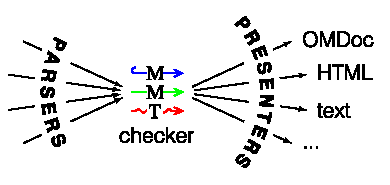
\includegraphics[scale=1.5]{parsers-mmt-presenters.pdf}
\caption{There can be many parsers and many presenters, but they all use the same \MMT checker}
\label{fig:mmtbottleneck}
\end{figure}

\section{Terms (2019-01-31)}
\label{sec:terms}

\textbf{Full session on YouTube:} \href{https://www.youtube.com/watch?v=vtePl2pGhfc}{Link}.
\bigskip

\begin{figure}[ht]
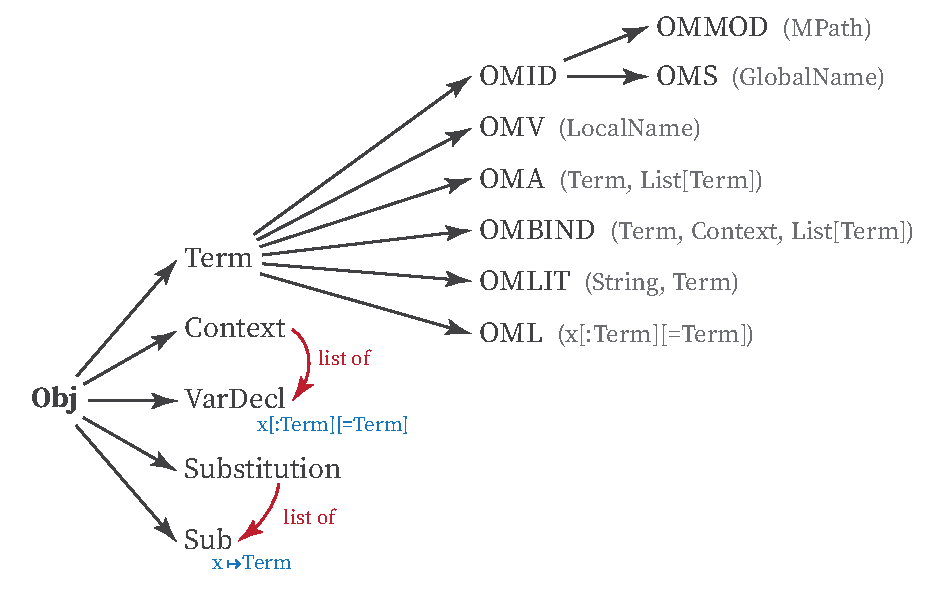
\includegraphics[scale=1]{mmt-terms.pdf}
\caption{Overview of \MMT Terms}
\label{fig:mmtterms}
\end{figure}


\end{document}